%% LyX 2.3.0 created this file.  For more info, see http://www.lyx.org/.
%% Do not edit unless you really know what you are doing.
\documentclass[british,english,showpacs,preprintnumbers,amssymb,aps,notitlepage]{revtex4-1}
\usepackage{lmodern}
\renewcommand{\sfdefault}{lmss}
\renewcommand{\ttdefault}{lmtt}
\usepackage[T1]{fontenc}
\usepackage[latin9]{inputenc}
\setcounter{secnumdepth}{3}
\usepackage{color}
\usepackage{array}
\usepackage{float}
\usepackage{multirow}
\usepackage{amsbsy}
\usepackage{graphicx}

\makeatletter

%%%%%%%%%%%%%%%%%%%%%%%%%%%%%% LyX specific LaTeX commands.
%% Binom macro for standard LaTeX users
\newcommand{\binom}[2]{{#1 \choose #2}}

%% Because html converters don't know tabularnewline
\providecommand{\tabularnewline}{\\}

%%%%%%%%%%%%%%%%%%%%%%%%%%%%%% User specified LaTeX commands.
\usepackage{amsfonts,amsmath} % amsmath added here instead to prevent clash with lyx function
% this is the preamble created by tikzit, we can edit this in the final document to change the shapes we use for nodes, edge styles, etc... 
% just be sure to use the same name for the same kind of node/edge in any figures you make


\usepackage[svgnames]{xcolor}
\usepackage{tikz}
\usetikzlibrary{decorations.markings}
\usetikzlibrary{shapes.geometric}
%\pagestyle{empty}

\newcommand\scaledLW{0.5} % scaled linewidth for fig 2, defined globally so they can be changed easily

\newcommand\scaledNodeSize{0.5} % scaled node size for fig 2, defined globally so they can be changed easily

\pgfdeclarelayer{edgelayer}
\pgfdeclarelayer{nodelayer}
\pgfsetlayers{edgelayer,nodelayer,main}

\tikzstyle{none}=[inner sep=0pt]

\tikzstyle{rn}=[circle,fill=Red,draw=Black,line width=0.8 pt]
\tikzstyle{gn}=[circle,fill=Lime,draw=Black,line width=0.8 pt]
\tikzstyle{yn}=[circle,fill=Yellow,draw=Black,line width=0.8 pt]
\tikzstyle{auxiliary_qubit}=[circle,fill=Red,draw=Black,scale=0.8]
\tikzstyle{logical_qubit}=[circle,fill=Black,draw=Black,scale=0.8]
\tikzstyle{emb_logical_qubit}=[circle,fill=Gray,draw=Black,scale=0.8,line width=2.000]
\tikzstyle{emb_auxiliary_qubit}=[circle,fill=Red,draw=Black,scale=0.8,line width=2.000]
\tikzstyle{unused_qubit}=[circle,fill=Gray,draw=Gray,scale=0.8]
\tikzstyle{arrow_end}=[circle,fill=none,draw=none,scale=.1]




\tikzstyle{simple}=[-,draw=Black,line width=1.000]
\tikzstyle{added}=[-,draw=Black,line width=1.000]
%\tikzstyle{added}=[-,draw=green,line width=1.000]
\definecolor{tempcolor}{rgb}{.9,.9,.9}
\tikzstyle{unused}=[-,draw=tempcolor,line width=0.500]
%\definecolor{tempcolor}{rgb}{.7,.9,.7}
%\tikzstyle{unused_added}=[-,draw=tempcolor,line width=1.000]
%\tikzstyle{unused_added}=[-,draw=green,draw opacity=1,line width=1.000,dashed]
%\tikzstyle{unused_added}=[-,draw=cyan,draw opacity=1,line width=0.5]
\tikzstyle{unused_added}=[-,draw=gray,draw opacity=1,line width=0.5]
\tikzstyle{embedding}=[-,draw=Black,line width=3.000]
\tikzstyle{arrow}=[-,draw=Black,postaction={decorate},decoration={markings,mark=at position .5 with {\arrow{>}}},line width=2.000]



\newcommand{\intextheight}{13 pt}
\let\fileinput\input % to allow conversion without turning tikz to lyx
\usepackage[font=small,labelfont=bf,
   justification=justified,
   singlelinecheck=false,
   format=plain]{caption}

\usepackage{threeparttable}
%\captionsetup[table]{
%  labelsep=newline,
%  justification=justified,
%  singlelinecheck=false,
%  textfont=it,
%}

\@ifundefined{showcaptionsetup}{}{%
 \PassOptionsToPackage{caption=false}{subfig}}
\usepackage{subfig}
\makeatother

\usepackage{babel}
\begin{document}

\title{Embedding quadratization gadgets on Chimera and Pegasus graphs}

\author{Nike Dattani}
\email{n.dattani@cfa.harvard.edu}

\selectlanguage{english}%

\affiliation{Harvard-Smithsonian Center for Astrophysics}

\author{Nicholas Chancellor}
\email{nicholas.chancellor@durham.ac.uk}

\selectlanguage{english}%

\affiliation{Durham University}
\begin{abstract}
We group all known quadratizations of cubic and quartic terms in
binary optimization problems into five and eight unique graphs respectively.
We then perform a minor embedding of these graphs onto the well-known
Chimera graph, and the brand new \emph{Pegasus} graph. In cases where
two or more graphs have a minor embedding with the same overhead in
terms of auxiliary variables, we make recommendations for which gadgets
are best to use for certain problems. 
\end{abstract}
\maketitle
Discrete optimization problems are often naturally formulated in terms
of minimizing some polynomial of degree $>2$ \citep{Dattani2014j},
which is then `quadratized' into a quadratic function which can be
solved using standard algorithms for universal classical computers
\citep{Kolmogorov}, using special-purpose classical annealers, or
using quantum annealers. With dozens of quadratization methods available
, one should choose the best quadratization for a given problem,
and for a given method for solving the problem. 

There are ways to quadratize functions of discrete variables without
adding any auxiliary variables \citep{Ishikawa2014,Tanburn2015a,Okada2015,Dridi2017},
but when those methods cannot be applied we introduce auxiliary variables.
The resulting quadratic functions (called `gadgets') that accurately
or exactly simulate the original high-degree functions, will have
some connectivity between the binary variables (or bits, or qubits,
herein referred to for convenience only, as qubits) which can be represented
by a graph in which vertices represent qubits and edges indicate when
two different qubits appear together in a quadratic term. Since this
graph incorporates no information about the linear terms, constant
term, or the coefficients of the quadratic terms, many different gadgets
have the same graph, therefore in this paper we will classify all
known quadratization gadgets into categories according to their corresponding
graph (herein called their `gadget graph'). 

\noindent 
\begin{figure}[h]
\caption{\label{fig:chimeraAndPegasus}Graph connectivities for D-Wave's Chimera
and Pegasus graphs.}

\subfloat[Chimera]{


\includegraphics[width=0.23\textwidth]{metapostfigs/fig_ChimeraTT}}~~~~\subfloat[Pegasus]{


\includegraphics[width=0.23\textwidth]{metapostfigs/fig_PegasusTT}}~~~~\subfloat[Chimera repeated]{

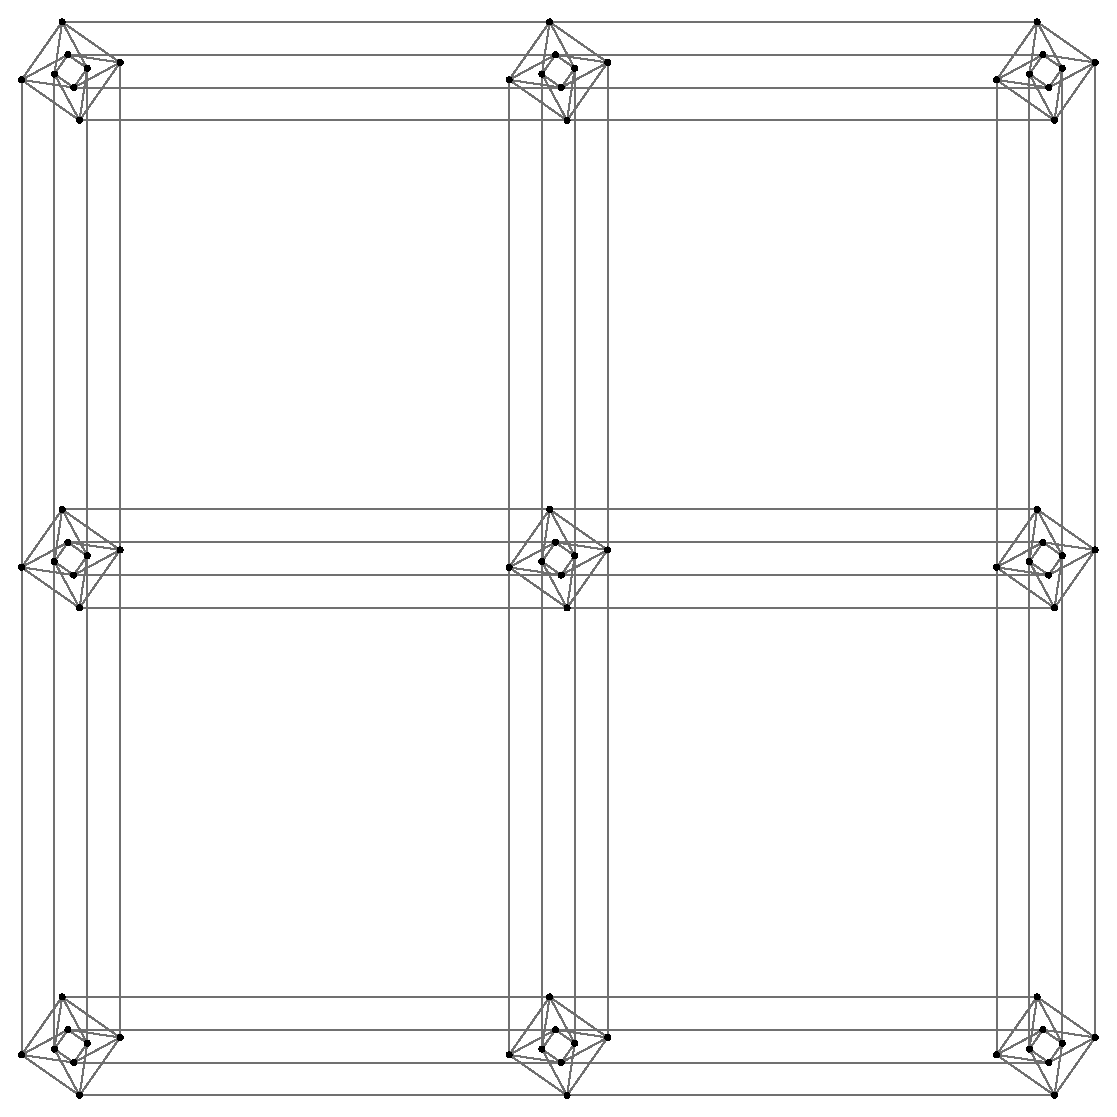
\includegraphics[width=0.23\textwidth]{metapostfigs/fig_ChimeraLL}}~~~~\subfloat[Pegasus repeated]{

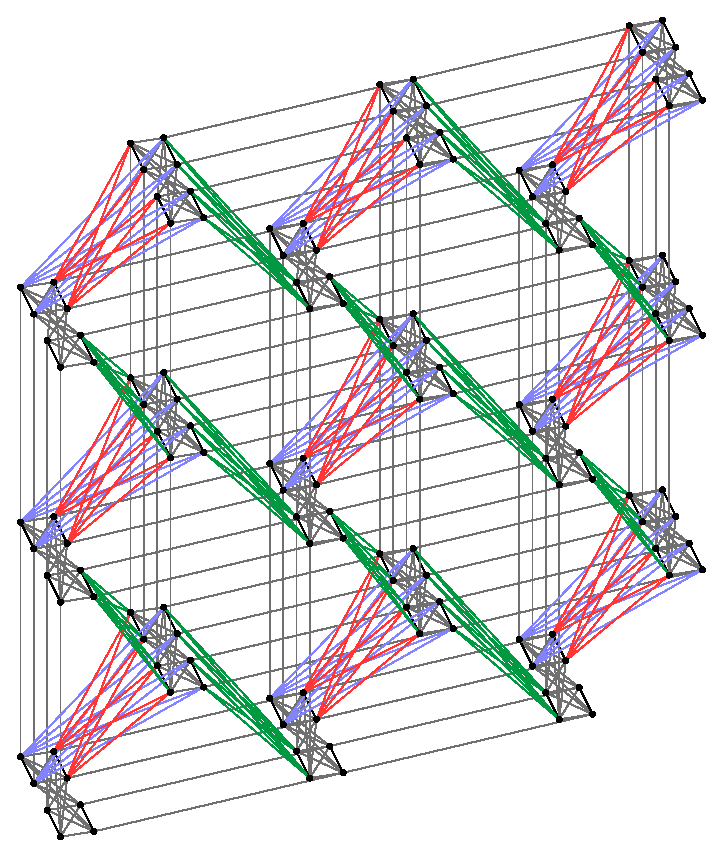
\includegraphics[width=0.23\textwidth]{metapostfigs/fig_PegasusLL}}
\end{figure}

\noindent 

\noindent 
\begin{figure}[h]
\caption{\label{fig:allGraphGadgets}Gadget graphs. Graphs showing the connectivity
between qubits in quadratization gadgets for cubic to quadratic gadgets
(top row), and quartic to quadratic gadgets (bottom row). Red vertices
represent auxiliary qubits and black vertices represent logical qubits.
Black edges denote the existence of a quadratic term in the gadget,
involving the two corresponding qubits represented by vertices connected
by the edge. \emph{Linear terms in the gadget are completely ignored
in these gadget graphs.}}

\newcommand{\thisfigheight}{1.5 cm}

\subfloat[``\emph{all to aux}'']{

\resizebox{!}{\thisfigheight}{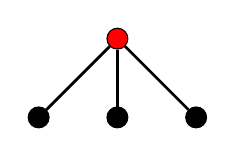
\begin{tikzpicture}
	\begin{pgfonlayer}{nodelayer}
		\node [style=auxiliary_qubit] (0) at (0, 5) {};
		\node [style=logical_qubit] (1) at (-1, 4) {};
		\node [style=logical_qubit] (2) at (0, 4) {};
		\node [style=logical_qubit] (3) at (1, 4) {};
	\end{pgfonlayer}
	\begin{pgfonlayer}{edgelayer}
		\draw [style=simple] (1) to (0);
		\draw [style=simple] (0) to (2);
		\draw [style=simple] (0) to (3);
	\end{pgfonlayer}
\end{tikzpicture}
}}\subfloat[$S_{3}$]{

\resizebox{!}{\thisfigheight}{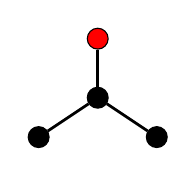
\begin{tikzpicture}
	\begin{pgfonlayer}{nodelayer}
		\node [style=logical_qubit] (0) at (0, -0) {};
		\node [style=auxiliary_qubit] (1) at (0, 0.75) {};
		\node [style=logical_qubit] (2) at (0.75, -0.5) {};
		\node [style=logical_qubit] (3) at (-0.75, -0.5) {};
	\end{pgfonlayer}
	\begin{pgfonlayer}{edgelayer}
		\draw [style=simple] (2) to (0);
		\draw [style=simple] (3) to (0);
		\draw [style=simple] (1) to (0);
	\end{pgfonlayer}
\end{tikzpicture}
 }}\subfloat[\mbox{``\emph{coat hanger}''}]{

\resizebox{!}{\thisfigheight}{\input{tikzit/k4_missing_2edge.tikz}
}}\subfloat[$K_{4}-1$]{

\resizebox{!}{\thisfigheight}{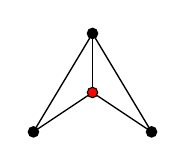
\begin{tikzpicture}[every node/.style={scale=\scaledNodeSize}]
	\begin{pgfonlayer}{nodelayer}
		\node [style=auxiliary_qubit] (0) at (0, -0) {};
		\node [style=logical_qubit] (1) at (0, 0.75) {};
		\node [style=logical_qubit] (2) at (0.75, -0.5) {};
		\node [style=logical_qubit] (3) at (-0.75, -0.5) {};
	\end{pgfonlayer}
	\begin{pgfonlayer}{edgelayer}
		\draw [style=simple,line width=\scaledLW] (3) to (1);
		\draw [style=simple,line width=\scaledLW] (1) to (2);
		\draw [style=simple,line width=\scaledLW] (2) to (0);
		\draw [style=simple,line width=\scaledLW] (3) to (0);
		\draw [style=simple,line width=\scaledLW] (1) to (0);
	\end{pgfonlayer}
\end{tikzpicture}

}}\subfloat[$K_{4}$]{

\resizebox{!}{\thisfigheight}{\input{tikzit/k4.tikz}}}

\subfloat[\emph{``all to aux''}]{

\resizebox{!}{\thisfigheight}{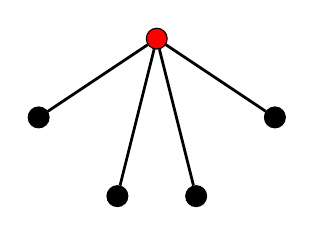
\begin{tikzpicture}
	\begin{pgfonlayer}{nodelayer}
		\node [style=logical_qubit] (0) at (-1, -0) {};
		\node [style=logical_qubit] (1) at (0, -1) {};
		\node [style=logical_qubit] (2) at (1, -1) {};
		\node [style=logical_qubit] (3) at (2, -0) {};
		\node [style=auxiliary_qubit] (4) at (0.5, 1) {};
	\end{pgfonlayer}
	\begin{pgfonlayer}{edgelayer}
		\draw [style=simple] (0) to (4);
		\draw [style=simple] (1) to (4);
		\draw [style=simple] (2) to (4);
		\draw [style=simple] (4) to (3);
	\end{pgfonlayer}
\end{tikzpicture}
}}\subfloat[``\emph{tripod}'']{

\resizebox{!}{\thisfigheight}{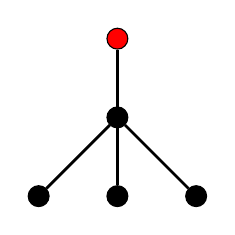
\begin{tikzpicture}
	\begin{pgfonlayer}{nodelayer}
		\node [style=logical_qubit] (0) at (0, -0) {};
		\node [style=auxiliary_qubit] (1) at (0, 1) {};
		\node [style=logical_qubit] (2) at (-1, -1) {};
		\node [style=logical_qubit] (3) at (1, -1) {};
		\node [style=logical_qubit] (4) at (0, -1) {};
	\end{pgfonlayer}
	\begin{pgfonlayer}{edgelayer}
		\draw [style=simple] (1) to (0);
		\draw [style=simple] (2) to (0);
		\draw [style=simple] (3) to (0);
		\draw [style=simple] (4) to (0);
	\end{pgfonlayer}
\end{tikzpicture}
}}\subfloat[``\emph{all to two aux + 1}'']{\resizebox{!}{\thisfigheight}{\input{tikzit/2aux_to_all4_1conn.tikz}}}\subfloat[\emph{$K_{6}$- 1}]{

\resizebox{!}{\thisfigheight}{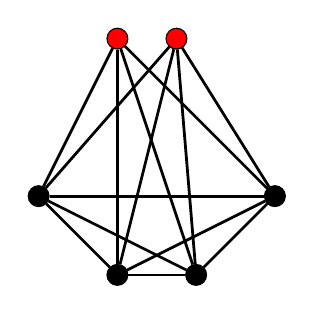
\begin{tikzpicture}
	\begin{pgfonlayer}{nodelayer}
		\node [style=logical_qubit] (0) at (-1, -0) {};
		\node [style=logical_qubit] (1) at (2, -0) {};
		\node [style=auxiliary_qubit] (2) at (0, 2) {};
		\node [style=auxiliary_qubit] (3) at (0.75, 2) {};
		\node [style=logical_qubit] (4) at (0, -1) {};
		\node [style=logical_qubit] (5) at (1, -1) {};
	\end{pgfonlayer}
	\begin{pgfonlayer}{edgelayer}
		\draw [style=simple] (2) to (1);
		\draw [style=simple] (0) to (3);
		\draw [style=simple] (3) to (1);
		\draw [style=simple] (4) to (1);
		\draw [style=simple] (0) to (2);
		\draw [style=simple] (5) to (3);
		\draw [style=simple] (5) to (4);
		\draw [style=simple] (5) to (2);
		\draw [style=simple] (5) to (1);
		\draw [style=simple] (4) to (3);
		\draw [style=simple] (4) to (2);
		\draw [style=simple] (4) to (0);
		\draw [style=simple] (0) to (5);
		\draw [style=simple] (0) to (1);
	\end{pgfonlayer}
\end{tikzpicture}

}}\subfloat[\emph{$K_{6}$}]{ 

\resizebox{!}{\thisfigheight}{\input{tikzit/2auxConn_to_all4_allConn.tikz}}}\subfloat[\emph{$K_{5}$}]{

\resizebox{!}{\thisfigheight}{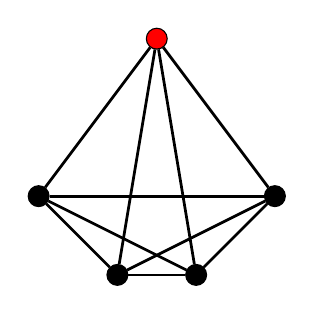
\begin{tikzpicture}
	\begin{pgfonlayer}{nodelayer}
		\node [style=logical_qubit] (0) at (2, -0) {};
		\node [style=auxiliary_qubit] (1) at (0.5, 2) {};
		\node [style=logical_qubit] (2) at (0, -1) {};
		\node [style=logical_qubit] (3) at (-1, -0) {};
		\node [style=logical_qubit] (4) at (1, -1) {};
	\end{pgfonlayer}
	\begin{pgfonlayer}{edgelayer}
		\draw [style=simple] (1) to (0);
		\draw [style=simple] (2) to (0);
		\draw [style=simple] (3) to (0);
		\draw [style=simple] (4) to (2);
		\draw [style=simple] (4) to (3);
		\draw [style=simple] (4) to (1);
		\draw [style=simple] (4) to (0);
		\draw [style=simple] (2) to (3);
		\draw [style=simple] (3) to (1);
		\draw [style=simple] (2) to (1);
	\end{pgfonlayer}
\end{tikzpicture}

}}\subfloat[\emph{$K_{5}$}+1]{

\resizebox{!}{\thisfigheight}{\input{tikzit/aux_to_all4_allConn_extra_qb.tikz}
}}\subfloat[``\emph{Double $K_{4}$}'']{

\resizebox{!}{\thisfigheight}{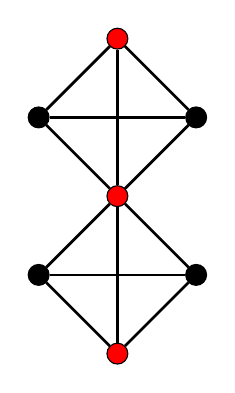
\begin{tikzpicture}
	\begin{pgfonlayer}{nodelayer}
		\node [style=logical_qubit] (0) at (-1, -0) {};
		\node [style=auxiliary_qubit] (1) at (0, 3) {};
		\node [style=logical_qubit] (2) at (-1, 2) {};
		\node [style=auxiliary_qubit] (3) at (0, 1) {};
		\node [style=logical_qubit] (4) at (1, -0) {};
		\node [style=auxiliary_qubit] (5) at (0, -1) {};
		\node [style=logical_qubit] (6) at (1, 2) {};
	\end{pgfonlayer}
	\begin{pgfonlayer}{edgelayer}
		\draw [style=simple] (2) to (1);
		\draw [style=simple] (3) to (1);
		\draw [style=simple] (4) to (0);
		\draw [style=simple] (0) to (5);
		\draw [style=simple] (4) to (5);
		\draw [style=simple] (6) to (3);
		\draw [style=simple] (6) to (2);
		\draw [style=simple] (6) to (1);
		\draw [style=simple] (2) to (3);
		\draw [style=simple] (0) to (3);
		\draw [style=simple] (4) to (3);
		\draw [style=simple] (5) to (3);
	\end{pgfonlayer}
\end{tikzpicture}
}}
\end{figure}

Gadget graphs for all known single cubic terms and for all known single
quartic terms are given in Figure \ref{fig:allGraphGadgets}. Gadget
graphs tell us a lot about how costly the quadratic optimization problem
will be, and those with larger connectivity tend to yield more difficult
functions to optimize. Furthermore, some optimization methods only
work if their corresponding graph has a certain connectivity, two
examples of such connectivities being the ones in D-Wave's well-known
Chimera graph, and in their very recently presented \emph{Pegasus}
graph, both shown in Figure. \ref{fig:chimeraAndPegasus}.

\begin{table}[b]
\caption{Grouping of all known quadratization gadgets for singe \textbf{\emph{cubic}}
terms, into categories corresponding to their gadget graphs. For each
unique gadget graph, the nuber of auxiliary qubits required for construction
of the gadget is listed, followed by the number of auxiliary qubits
required to minor-embed the gadget graph onto Chimera and Pegasus.}

\rule{1\columnwidth}{0.5pt}

\begin{tabular*}{1\columnwidth}{@{\extracolsep{\fill}}ccccccccccc}
\hline 
\noalign{\vskip2mm}
\multirow{3}{*}{Gadget Graph} & \multirow{3}{*}{Example Gadgets} & \multirow{2}{*}{} & $N_{{\rm aux}}$ &  & $N_{{\rm aux}}$  & $N_{{\rm aux}}$  &  &  & $N_{{\rm aux}}$  & $N_{{\rm aux}}$ \tabularnewline
 &  &  & \textbf{\scriptsize{}Quadratization} & \multirow{2}{*}{} & \textbf{\scriptsize{}Embedding} & \textbf{\scriptsize{}Total} &  &  & \textbf{\scriptsize{}Embedding} & \textbf{\scriptsize{}Total}\tabularnewline[2mm]
\cline{6-7} \cline{10-11} 
\noalign{\vskip2mm}
 &  &  &  &  & \multicolumn{2}{c}{\textbf{\textcolor{black}{Chimera}}} &  &  & \multicolumn{2}{c}{\textbf{\textcolor{black}{Pegasus}}}\tabularnewline[2mm]
\hline 
\noalign{\vskip2mm}
\multicolumn{4}{c}{Cubic $\rightarrow$ Quadratic} &  & \tabularnewline[2mm]
\hline 
\hline 
\noalign{\vskip2mm}
\multirow{2}{*}{\textbf{\textcolor{blue}{All to Aux}}} & NTR-KZFD &  & \multirow{2}{*}{1} &  & \multirow{2}{*}{0} & \multirow{2}{*}{\textbf{\textcolor{red}{1}}} &  &  & \multirow{2}{*}{0} & \multirow{2}{*}{\textbf{\textcolor{red}{1}}}\tabularnewline
 & NTR-ABCG &  &  &  &  &  &  &  &  & \tabularnewline[2mm]
\hline 
\noalign{\vskip2mm}
\textbf{\textcolor{blue}{$\boldsymbol{\textcolor{blue}{\ensuremath{S_{3}}}}$}} & NTR-ABCB &  & 1 &  & 0 & \textbf{\textcolor{red}{1}} &  &  & 0 & \textbf{\textcolor{red}{1}}\tabularnewline[2mm]
\hline 
\noalign{\vskip2mm}
\textbf{\textcolor{blue}{Coat Hanger}} & PTR-A &  & 1 &  & 1 & \textbf{\textcolor{red}{2}} &  &  & 0 & \textbf{\textcolor{red}{1}}\tabularnewline[2mm]
\hline 
\noalign{\vskip2mm}
\textbf{\textcolor{blue}{$\textcolor{blue}{\ensuremath{\boldsymbol{K_{4}}}-1}$}} & NTR-AC &  & 1 &  & 1 & \textbf{\textcolor{red}{2}} &  &  & 0 & \textbf{\textcolor{red}{1}}\tabularnewline[2mm]
\hline 
\noalign{\vskip2mm}
\multirow{4}{*}{\textbf{\textcolor{blue}{$\textcolor{blue}{\ensuremath{\boldsymbol{K_{4}}}}$}}} & PTR-Ishikawa &  & \multirow{4}{*}{1} &  & \multirow{4}{*}{2} & \multirow{4}{*}{\textbf{\textcolor{red}{3}}} & \multirow{4}{*}{} & \multirow{1}{*}{} & \multirow{4}{*}{0} & \multirow{4}{*}{\textbf{\textcolor{red}{1}}}\tabularnewline
 & NTR-RBL-(3$\rightarrow2$) &  &  &  &  &  &  & \multirow{3}{*}{} &  & \tabularnewline
 & PTR-BCR-1,2,3,4 &  &  &  &  &  &  &  &  & \tabularnewline
 & PTR-KZ &  &  &  &  &  &  &  &  & \tabularnewline[2mm]
\hline 
\noalign{\vskip2mm}
\textbf{\textcolor{blue}{$K_{5}$+1}} & PTR-RBL-(3$\rightarrow2$) &  & 3 &  & 5 & \textbf{\textcolor{red}{8}} &  &  & 1 & \textbf{\textcolor{red}{4}}\tabularnewline[2mm]
\hline 
\end{tabular*}

\rule{1\columnwidth}{0.5pt}
\end{table}

\begin{table}[b]
\caption{Grouping of all known quadratization gadgets for single \textbf{\emph{quartic}}
terms, into categories corresponding to their gadget graphs. For each
unique gadget graph, the nuber of auxiliary qubits required for construction
of the gadget is listed, followed by the number of auxiliary qubits
required to minor-embed the gadget graph onto Chimera and Pegasus.}

\rule{1\columnwidth}{0.5pt}

\begin{tabular*}{1\columnwidth}{@{\extracolsep{\fill}}ccccccccccc}
\hline 
\noalign{\vskip2mm}
\multirow{3}{*}{Gadget Graph} & \multirow{3}{*}{Example Gadgets} & \multirow{2}{*}{} & $N_{{\rm aux}}$ &  & $N_{{\rm aux}}$  & $N_{{\rm aux}}$  &  &  & $N_{{\rm aux}}$  & $N_{{\rm aux}}$ \tabularnewline
 &  &  & \textbf{\scriptsize{}Quadratization} & \multirow{2}{*}{} & \textbf{\scriptsize{}Embedding} & \textbf{\scriptsize{}Total} &  &  & \textbf{\scriptsize{}Embedding} & \textbf{\scriptsize{}Total}\tabularnewline[2mm]
\cline{6-7} \cline{10-11} 
\noalign{\vskip2mm}
 &  &  &  &  & \multicolumn{2}{c}{\textbf{\textcolor{black}{Chimera}}} &  &  & \multicolumn{2}{c}{\textbf{\textcolor{black}{Pegasus}}}\tabularnewline[2mm]
\hline 
\hline 
\noalign{\vskip2mm}
\textbf{\textcolor{blue}{All to Aux}} & NTR-KZFD &  & 1 &  & 0 & \textbf{\textcolor{red}{1}} &  &  & 0 & \textbf{\textcolor{red}{1}}\tabularnewline[2mm]
\hline 
\noalign{\vskip2mm}
\textbf{\textcolor{blue}{Tripod}} & NTR-ABCB &  & 1 &  & 0 & \textbf{\textcolor{red}{1}} &  &  & 0 & \textbf{\textcolor{red}{1}}\tabularnewline[2mm]
\hline 
\noalign{\vskip2mm}
\textbf{\textcolor{blue}{All22Aux+1}} & PTR &  & 2 &  & 1 & \textbf{\textcolor{red}{3}} &  &  & 0 & \textbf{\textcolor{red}{2}}\tabularnewline[2mm]
\hline 
\noalign{\vskip2mm}
\textbf{\textcolor{blue}{All2All - 1}} & PTR-Ishikawa &  & 2 &  & 5 & \textbf{\textcolor{red}{7}} &  &  & 2 & \textbf{\textcolor{red}{4}}\tabularnewline[2mm]
\hline 
\noalign{\vskip2mm}
\multirow{3}{*}{\textbf{\textcolor{blue}{$K_{5}$}}} & PTR-BCR-2 &  & \multirow{3}{*}{1} &  & \multirow{3}{*}{3} & \multirow{3}{*}{\textbf{\textcolor{red}{4}}} &  &  & \multirow{3}{*}{2} & \multirow{3}{*}{\textbf{\textcolor{red}{3}}}\tabularnewline
 & PTR-BCR-4 &  &  &  &  &  &  &  &  & \tabularnewline
 & NTR-RBL-(4$\rightarrow2$) &  &  &  &  &  &  &  &  & \tabularnewline[2mm]
\hline 
\noalign{\vskip2mm}
\multirow{1}{*}{\textbf{\textcolor{blue}{$K_{6}$}}} & \multirow{1}{*}{PTR-BCR-3} & \multirow{1}{*}{} & \multirow{1}{*}{2} &  & \multirow{1}{*}{8} & \multirow{1}{*}{\textbf{\textcolor{red}{10}}} &  &  & \multirow{1}{*}{2} & \multirow{1}{*}{\textbf{\textcolor{red}{4}}}\tabularnewline[2mm]
\hline 
\noalign{\vskip2mm}
\textbf{\textcolor{blue}{Double $K_{4}$}} & PTR-KZ(?) &  & 3 &  & 5 & \textbf{\textcolor{red}{8}} &  &  & 1 & \textbf{\textcolor{red}{4}}\tabularnewline[2mm]
\hline 
\end{tabular*}

\rule{1\columnwidth}{0.5pt}
\end{table}

\begin{figure}
\caption{\label{fig:ChimeraAndPegasus}}
\end{figure}

Any graph, can be mapped onto the Chimera or Pegasus graphs by minor-embedding
\citep{Choi2008,Choi2011}, where the Chimera graph or the Pegasus
graph is a graph minor of the graph representing the problem that
needs to be optimized. This often means that one binary variable in
the quadratic optimization problem needs to be represented by two
qubits instead of one, making the number of qubits needed to solve
the original problem larger than before, and sometimes completely
impossible. For example a quartic function with 1000 binary variables
has $\binom{1000}{3}>166$ million possible cubic terms and $\binom{1000}{4}>40$
billion possible quartic terms which have to be quadratized, and then
minor-embedded. If our minimization method can only be applied for
up to 50 billion qubits, we cannot afford for each quartic-to-quadratic
gadget to require its own auxiliary qubit for minor-embedding.

We have provided minor-embeddings for all gadget graphs in Figure
\ref{fig:allGraphGadgets}, for both Chimera and Pegasus. We note
that \textbf{\emph{all}} cubic to quadratic gadgets involvnig one
auxiliary qubit can be embedded onto Pegasus without any further auxiliary
qubits for the embedding, because Pegasus contains the $K_{4}$ graph,
which means any possible connections between the three logical qubits
and the one auxiliary qubit are already contained in Pegasus. Since
Chimera does not contain $K_{4}$, only negative cubic terms are so
far known to be quadratizable with gadgets that embed directly onto
Chimera without any extra qubits for the embedding.

\section{Minor embeddings for cubic to quadratic gadgets}

\subsection{Chimera graph}

\begin{figure}[H]
\caption{Minor embeddings of all \textbf{\emph{cubic }}to quadratic gadgets
onto a `unit cell' of a Chimera graph. Grey vertices and edges are
not used. Thick black edges denote graph minors, in which two physical
qubits (two vertices) represent one logical qubit (this is done when
logical qubits need to be connected to more qubits than the Chimera
unit cell otherwise allows).}

\newcommand{\chimeraFigSize}{3cm}
\centering{}\subfloat[``\emph{all to aux''\label{fig:all-to-auxChimera}}]{\resizebox{!}{\chimeraFigSize}{\input{tikzit/all_to_aux_chimera.tikz}}}~~~\subfloat[``\emph{Y''\label{fig:Ychimera}}]{\resizebox{!}{\chimeraFigSize}{\input{tikzit/logical_fork_chimera.tikz}}}~~~\subfloat[``\emph{coat hanger''}]{\resizebox{!}{\chimeraFigSize}{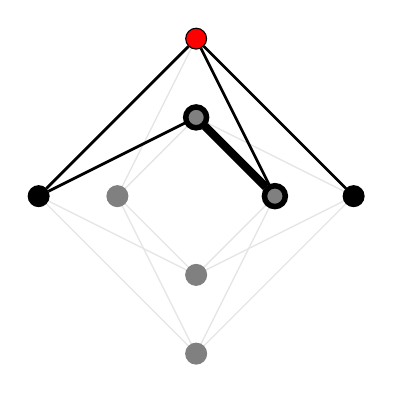
\begin{tikzpicture}
	\begin{pgfonlayer}{nodelayer}
		\node [style={logical_qubit}] (0) at (-2, 0) {};
		\node [style={unused_qubit}] (1) at (-1, 0) {};
		\node [style={logical_qubit}] (2) at (2, 0) {};
		\node [style={emb_logical_qubit}] (3) at (0, 1) {};
		\node [style={unused_qubit}] (4) at (0, -1) {};
		\node [style={unused_qubit}] (5) at (0, -2) {};
		\node [style={emb_logical_qubit}] (6) at (1, 0) {};
		\node [style={auxiliary_qubit}] (7) at (0, 2) {};
	\end{pgfonlayer}
	\begin{pgfonlayer}{edgelayer}
		\draw [style=unused] (1) to (3);
		\draw [style=unused] (3) to (2);
		\draw [style=unused] (1) to (4);
		\draw [style=unused] (4) to (2);
		\draw [style=unused] (4) to (0);
		\draw [style=unused] (0) to (5);
		\draw [style=unused] (5) to (2);
		\draw [style=unused] (5) to (1);
		\draw [style=embedding] (6) to (3);
		\draw [style=unused] (6) to (4);
		\draw [style=unused] (6) to (5);
		\draw [style=simple] (0) to (7);
		\draw [style=simple] (6) to (7);
		\draw [style=simple] (7) to (2);
		\draw [style=unused] (1) to (7);
		\draw [style=simple] (0) to (3);
	\end{pgfonlayer}
\end{tikzpicture}
}}~~~\subfloat[``\textcolor{black}{$K_{5}$}\emph{''}]{\resizebox{!}{\chimeraFigSize}{\input{tikzit/aux_to_all4_allConn_inChimera.tikz}}}~~~\subfloat[``\emph{all to all''}]{\resizebox{!}{\chimeraFigSize}{\input{tikzit/k4_chimera.tikz}}}
\end{figure}


\subsection{Pegasus graph}

\begin{figure}[H]
\caption{Minor embeddings of all \textbf{\emph{cubic }}to quadratic gadgets
onto a `unit cell' of a Pegasus graph. Grey vertices and edges are
not used. Figures \ref{fig:all-to-auxChimera} and \ref{fig:Ychimera}
do not need to be altered since the Chimera graph is a sub-graph of
Pegasus, so only the gadgets that required auxiliary qubits for minor
embedding onto Chimera are embedded for Pegasus here to show that
with Pegasus no auxiliary qubits are needed for cubic to quadratic
gadgets.}

\newcommand{\chimeraFigSize}{3cm}
\centering{}\subfloat[``\emph{coat hanger''}]{\resizebox{!}{\chimeraFigSize}{\input{tikzit/k4_missing_2edge_pegasus.tikz}
}}~~~\subfloat[``\emph{''}]{\resizebox{!}{\chimeraFigSize}{\input{tikzit/k4_missing_edge_pegasus.tikz}
}}~~~\subfloat[``\emph{all to all''}]{\resizebox{!}{\chimeraFigSize}{\input{tikzit/k4_pegasus.tikz} }}\subfloat[``\emph{all to all''}]{\resizebox{!}{\chimeraFigSize}{\input{tikzit/k4_pegasus.tikz} }}
\end{figure}


\section{Minor embeddings for quartic to quadratic gadgets}

\subsection{Chimera graph}

\begin{figure}[H]
\caption{Minor embeddings of all \textbf{\emph{quartic}} to quadratic gadgets
onto a `unit cell' of a Chimera graph. Grey vertices and edges are
not used. Thick black edges denote graph minors, in which two physical
qubits (two vertices) represent one logical qubit (this is done when
logical qubits need to be connected to more qubits than the Chimera
unit cell otherwise allows).}

\newcommand{\chimeraFigSize}{2.5cm}
\centering{}\subfloat[``\emph{all to aux''\label{fig:all-to-auxChimera-1}}]{\resizebox{!}{\chimeraFigSize}{\input{tikzit/all_to_aux4_inChimera.tikz}
}}~~~\subfloat[``\textcolor{black}{Tripod}\emph{''\label{fig:Ychimera-1}}]{\resizebox{!}{\chimeraFigSize}{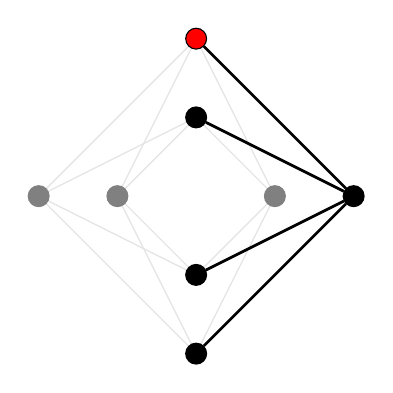
\begin{tikzpicture}
	\begin{pgfonlayer}{nodelayer}
		\node [style=unused_qubit] (0) at (-2, -0) {};
		\node [style=unused_qubit] (1) at (-1, -0) {};
		\node [style=logical_qubit] (2) at (2, -0) {};
		\node [style=auxiliary_qubit] (3) at (0, 2) {};
		\node [style=logical_qubit] (4) at (0, 1) {};
		\node [style=logical_qubit] (5) at (0, -1) {};
		\node [style=logical_qubit] (6) at (0, -2) {};
		\node [style=unused_qubit] (7) at (1, -0) {};
	\end{pgfonlayer}
	\begin{pgfonlayer}{edgelayer}
		\draw [style=unused] (1) to (4);
		\draw [style=unused] (0) to (4);
		\draw [style=unused] (5) to (0);
		\draw [style=unused] (0) to (6);
		\draw [style=unused] (1) to (5);
		\draw [style=unused] (0) to (3);
		\draw [style=unused] (1) to (3);
		\draw [style=unused] (7) to (4);
		\draw [style=unused] (7) to (5);
		\draw [style=unused] (7) to (6);
		\draw [style=unused] (7) to (3);
		\draw [style=unused] (6) to (1);
		\draw [style=simple] (3) to (2);
		\draw [style=simple] (4) to (2);
		%\draw [style={unused_added}] (0) to (1);
		\draw [style=simple] (5) to (2);
		\draw [style=simple] (6) to (2);
		%\draw [style={unused_added}] (3) to (4);
		%\draw [style={unused_added}] (5) to (6);
		%\draw [style={unused_added}] (7) to (2);
	\end{pgfonlayer}
\end{tikzpicture}

}}~~~\subfloat[``\textcolor{black}{All22Aux+1}\emph{''}]{\resizebox{!}{\chimeraFigSize}{\input{tikzit/2aux_to_all4_1conn_inChimera.tikz}
}}~~~\subfloat[``\textcolor{black}{$K_{5}$}\emph{''}]{\resizebox{!}{\chimeraFigSize}{\input{tikzit/aux_to_all4_allConn_inChimera.tikz}
}}
\end{figure}


\subsection{Pegasus graph}

\begin{figure}[H]
\caption{Minor embeddings of all \textbf{\emph{quartic}} to quadratic gadgets
onto a `unit cell' of a Pegasus graph. Grey vertices and edges are
not used. }

\newcommand{\chimeraFigSize}{2.5cm}
\centering{}\subfloat[``\emph{all to aux''}]{\resizebox{!}{\chimeraFigSize}{\input{tikzit/all_to_aux4_inPegasus.tikz}}}\subfloat[``\emph{''}]{\resizebox{!}{\chimeraFigSize}{\input{tikzit/logical_fork3_inPegasus.tikz}}}\subfloat[``\emph{all to all''}]{\resizebox{!}{\chimeraFigSize}{\input{tikzit/2aux_to_all4_1conn_inPegasus.tikz}}}\subfloat[``\textbf{\textcolor{black}{$K_{5}$+1}}\emph{''}]{\resizebox{!}{\chimeraFigSize}{\input{tikzit/aux_to_all4_allConn_inPegasus_extra_qb.tikz}
}}\subfloat[``\emph{$K_{6}$''}]{\resizebox{!}{\chimeraFigSize}{\input{tikzit/2auxConn_to_all4_allConn_inPegasus.tikz}}}\subfloat[``\emph{$K_{5}$''}]{\resizebox{!}{\chimeraFigSize}{\input{tikzit/aux_to_all4_allConn_inPegasus.tikz}
}}\subfloat[``\emph{Two $K_{4}'s$''}]{\resizebox{!}{\chimeraFigSize}{\input{tikzit/2k4_shared_aux_inPegasus.tikz}}}
\end{figure}


\section{Recommended gadgets}

All gadgets described in this work for quadratizing negative terms
(whether cubic or quartic) can be quadratized with only one auxiliary
qubit, and can be chimerized and pegasized wihout any futher auxiliary
qubits. On Pegasus, there is one 4-local to 2-local gadget for positive
terms which stands out over the rest, and it is PTR (which has the
``all22aux+1'' gadget graph). This is the \emph{only }gadget which
embeds positive quartic terms onto Pegasus with only two total auxiliaries
(two for the quadratization, and none for the embedding onto the Pegasus
graph). All other gadgets for positive quartic terms require three
or four total auxiliaries to embed onto Pegasus. 

\selectlanguage{british}%
\bibliographystyle{apsrev4-1}
\bibliography{\string"/home/nike/pCloud Sync/library\string"}
\selectlanguage{english}%

\end{document}
